\section{Definição}

\begin{frame}[fragile]{Travessia de um grafo}

    \begin{itemize}
        \item Uma travessia de um grafo consiste em visitar todos os nós alcançáveis a partir
            de um nó inicial $s$

        \item Cada nó deve ser processado uma única vez, embora a travessia possar passar por um
            nó mais de uma vez

        \item Uma travessia $T_1$ é diferente de uma travessia $T_2$ se ambas diferem na ordem de
            visitação dos vértices

        \item Um grafo conectado com $N$ nós tem $N!$ travessias possíveis

        \item Dentre todas estas travessias, duas se destacam pela aplicabilidade em situações
            práticas: a travessia por profundidade e a travessia por largura.
    \end{itemize}

\end{frame}

\begin{frame}[fragile]{\textit{Depth-First Search}}

    \begin{itemize}
        \item A travessia por profundidade (\textit{Depth-First Search -- DFS}) segue, a partir
            do nó inicial $s$, um caminho único, enquanto encontrar novos nós

        \item Quando não for possível encontrar novos nós, a DFS retorna ao nó anterior e 
            retoma o caminho usando o próximo nó encontrado

        \item A DFS mantém um registro dos nós visitados, de forma que cada nó seja processado
            uma única vez

        \item Em um grafo conectado com $N$ nós e $M$ arestas, a complexidade da DFS é
            $O(N + M)$, pois cada nó e cada aresta é processada uma única vez

        \item Se o grafo for representado como matrizes de adjacências, a complexidade é 
            $O(N^2)$

    \end{itemize}

\end{frame}

\begin{frame}[fragile]{Visualização da DFS}

    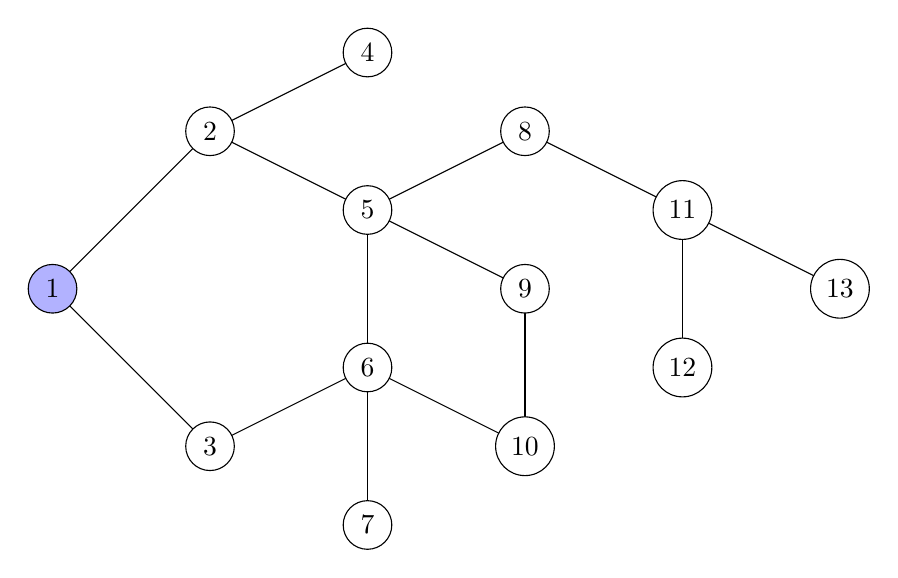
\begin{tikzpicture}
        \draw (0,4) -- (2,6);
        \draw (0,4) -- (2,2);
        \draw (2,6) -- (4,7);
        \draw (2,6) -- (4,5);
        \draw (4,5) -- (4,3);
        \draw (4,3) -- (2,2);
        \draw (4,3) -- (4,1);
        \draw (4,3) -- (6,2);
        \draw (4,5) -- (6,6);
        \draw (4,5) -- (6,4);
        \draw (6,2) -- (6,4);
        \draw (6,6) -- (8,5);
        \draw (8,5) -- (8,3);
        \draw (8,5) -- (10,4);

        \node[circle, draw, fill=blue!30] at (0, 4) {1};
        \node[circle, draw, fill=white] at (2, 6) {2};
        \node[circle, draw, fill=white] at (2, 2) {3};
        \node[circle, draw, fill=white] at (4, 7) {4};
        \node[circle, draw, fill=white] at (4, 5) {5};
        \node[circle, draw, fill=white] at (4, 3) {6};
        \node[circle, draw, fill=white] at (4, 1) {7};
        \node[circle, draw, fill=white] at (6, 6) {8};
        \node[circle, draw, fill=white] at (6, 4) {9};
        \node[circle, draw, fill=white] at (6, 2) {10};
        \node[circle, draw, fill=white] at (8, 5) {11};
        \node[circle, draw, fill=white] at (8, 3) {12};
        \node[circle, draw, fill=white] at (10, 4) {13};

    \end{tikzpicture}

\end{frame}

\begin{frame}[fragile]{Visualização da DFS}

    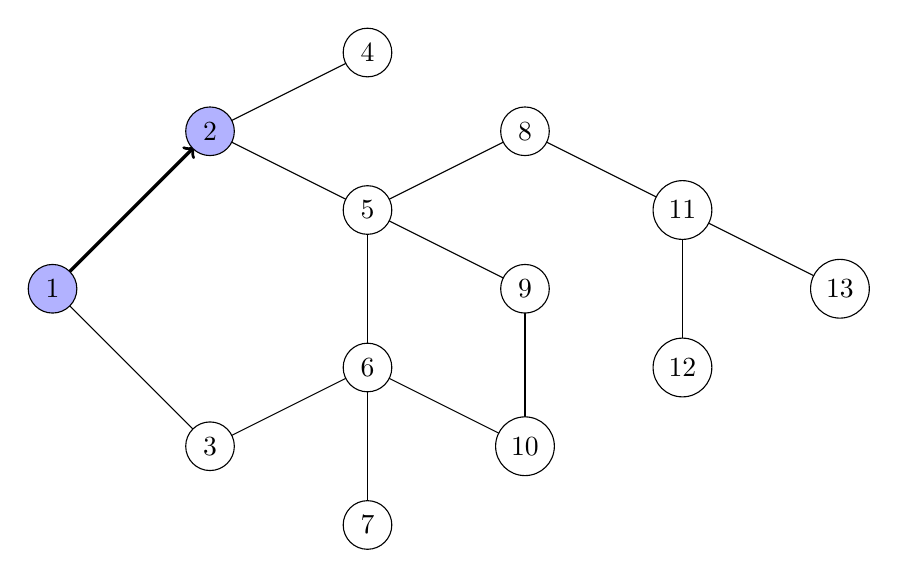
\begin{tikzpicture}
        \draw[very thick,->] (0,4) -- (1.8,5.8);
        \draw (0,4) -- (2,2);
        \draw (2,6) -- (4,7);
        \draw (2,6) -- (4,5);
        \draw (4,5) -- (4,3);
        \draw (4,3) -- (2,2);
        \draw (4,3) -- (4,1);
        \draw (4,3) -- (6,2);
        \draw (4,5) -- (6,6);
        \draw (4,5) -- (6,4);
        \draw (6,2) -- (6,4);
        \draw (6,6) -- (8,5);
        \draw (8,5) -- (8,3);
        \draw (8,5) -- (10,4);

        \node[circle, draw, fill=blue!30] at (0, 4) {1};
        \node[circle, draw, fill=blue!30] at (2, 6) {2};
        \node[circle, draw, fill=white] at (2, 2) {3};
        \node[circle, draw, fill=white] at (4, 7) {4};
        \node[circle, draw, fill=white] at (4, 5) {5};
        \node[circle, draw, fill=white] at (4, 3) {6};
        \node[circle, draw, fill=white] at (4, 1) {7};
        \node[circle, draw, fill=white] at (6, 6) {8};
        \node[circle, draw, fill=white] at (6, 4) {9};
        \node[circle, draw, fill=white] at (6, 2) {10};
        \node[circle, draw, fill=white] at (8, 5) {11};
        \node[circle, draw, fill=white] at (8, 3) {12};
        \node[circle, draw, fill=white] at (10, 4) {13};

    \end{tikzpicture}

\end{frame}

\begin{frame}[fragile]{Visualização da DFS}

    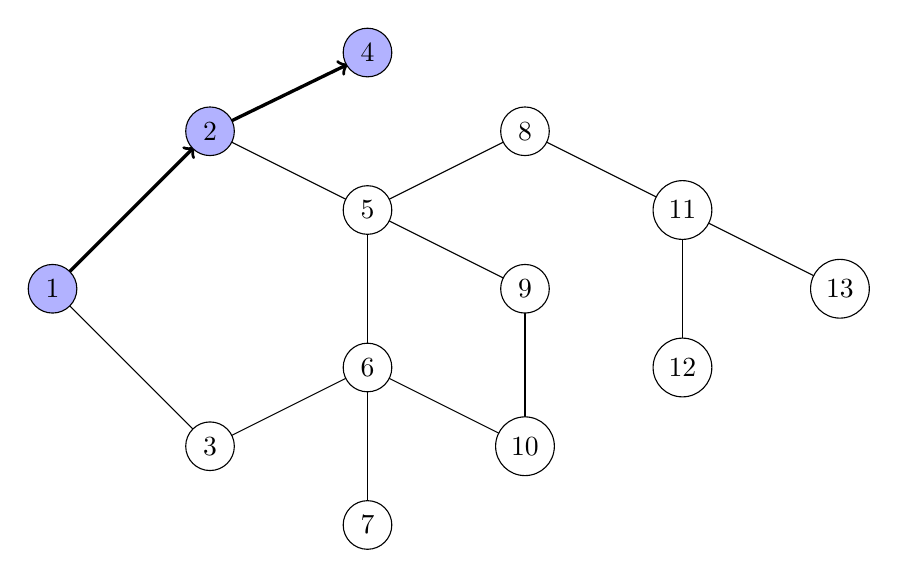
\begin{tikzpicture}
        \draw[very thick,->] (0,4) -- (1.8,5.8);
        \draw[very thick,->] (2,6) -- (3.75,6.85);
        \draw (0,4) -- (2,2);
        \draw (2,6) -- (4,5);
        \draw (4,5) -- (4,3);
        \draw (4,3) -- (2,2);
        \draw (4,3) -- (4,1);
        \draw (4,3) -- (6,2);
        \draw (4,5) -- (6,6);
        \draw (4,5) -- (6,4);
        \draw (6,2) -- (6,4);
        \draw (6,6) -- (8,5);
        \draw (8,5) -- (8,3);
        \draw (8,5) -- (10,4);

        \node[circle, draw, fill=blue!30] at (0, 4) {1};
        \node[circle, draw, fill=blue!30] at (2, 6) {2};
        \node[circle, draw, fill=white] at (2, 2) {3};
        \node[circle, draw, fill=blue!30] at (4, 7) {4};
        \node[circle, draw, fill=white] at (4, 5) {5};
        \node[circle, draw, fill=white] at (4, 3) {6};
        \node[circle, draw, fill=white] at (4, 1) {7};
        \node[circle, draw, fill=white] at (6, 6) {8};
        \node[circle, draw, fill=white] at (6, 4) {9};
        \node[circle, draw, fill=white] at (6, 2) {10};
        \node[circle, draw, fill=white] at (8, 5) {11};
        \node[circle, draw, fill=white] at (8, 3) {12};
        \node[circle, draw, fill=white] at (10, 4) {13};

    \end{tikzpicture}

\end{frame}

\begin{frame}[fragile]{Visualização da DFS}

    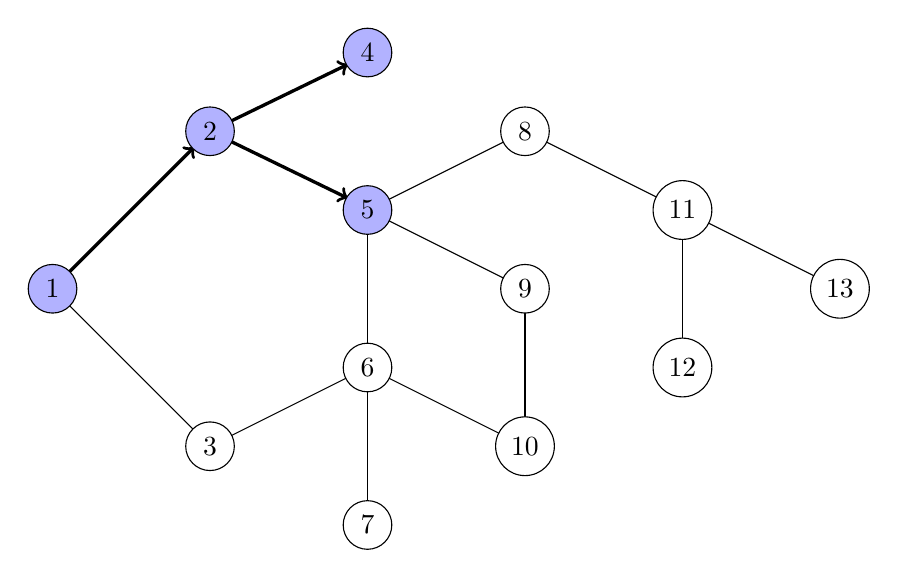
\begin{tikzpicture}
        \draw[very thick,->] (0,4) -- (1.8,5.8);
        \draw[very thick,->] (2,6) -- (3.75,6.85);
        \draw[very thick,->] (2,6) -- (3.75,5.15);
        \draw (0,4) -- (2,2);
        \draw (4,5) -- (4,3);
        \draw (4,3) -- (2,2);
        \draw (4,3) -- (4,1);
        \draw (4,3) -- (6,2);
        \draw (4,5) -- (6,6);
        \draw (4,5) -- (6,4);
        \draw (6,2) -- (6,4);
        \draw (6,6) -- (8,5);
        \draw (8,5) -- (8,3);
        \draw (8,5) -- (10,4);

        \node[circle, draw, fill=blue!30] at (0, 4) {1};
        \node[circle, draw, fill=blue!30] at (2, 6) {2};
        \node[circle, draw, fill=white] at (2, 2) {3};
        \node[circle, draw, fill=blue!30] at (4, 7) {4};
        \node[circle, draw, fill=blue!30] at (4, 5) {5};
        \node[circle, draw, fill=white] at (4, 3) {6};
        \node[circle, draw, fill=white] at (4, 1) {7};
        \node[circle, draw, fill=white] at (6, 6) {8};
        \node[circle, draw, fill=white] at (6, 4) {9};
        \node[circle, draw, fill=white] at (6, 2) {10};
        \node[circle, draw, fill=white] at (8, 5) {11};
        \node[circle, draw, fill=white] at (8, 3) {12};
        \node[circle, draw, fill=white] at (10, 4) {13};

    \end{tikzpicture}

\end{frame}

\begin{frame}[fragile]{Visualização da DFS}

    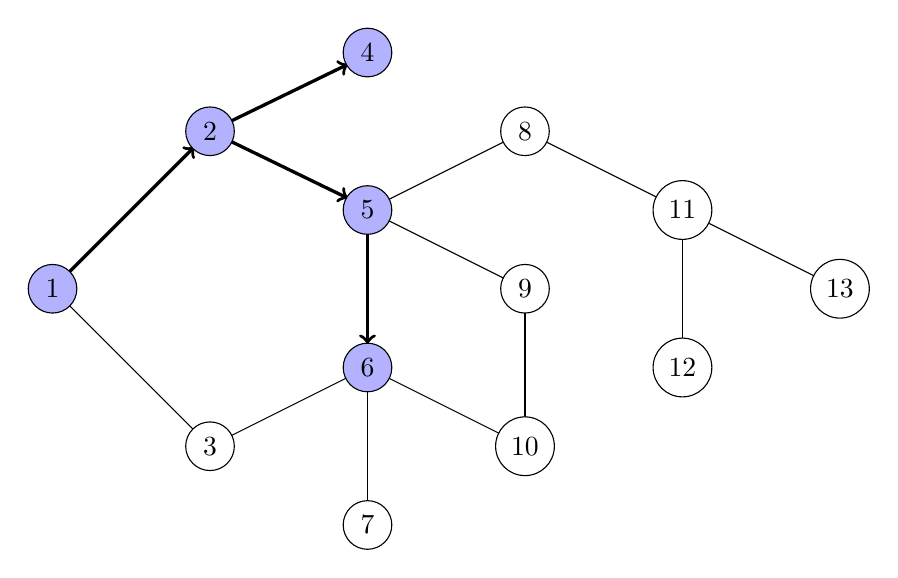
\begin{tikzpicture}
        \draw[very thick,->] (0,4) -- (1.8,5.8);
        \draw[very thick,->] (2,6) -- (3.75,6.85);
        \draw[very thick,->] (2,6) -- (3.75,5.15);
        \draw[very thick,->] (4,5) -- (4,3.3);
        \draw (0,4) -- (2,2);
        \draw (4,3) -- (2,2);
        \draw (4,3) -- (4,1);
        \draw (4,3) -- (6,2);
        \draw (4,5) -- (6,6);
        \draw (4,5) -- (6,4);
        \draw (6,2) -- (6,4);
        \draw (6,6) -- (8,5);
        \draw (8,5) -- (8,3);
        \draw (8,5) -- (10,4);

        \node[circle, draw, fill=blue!30] at (0, 4) {1};
        \node[circle, draw, fill=blue!30] at (2, 6) {2};
        \node[circle, draw, fill=white] at (2, 2) {3};
        \node[circle, draw, fill=blue!30] at (4, 7) {4};
        \node[circle, draw, fill=blue!30] at (4, 5) {5};
        \node[circle, draw, fill=blue!30] at (4, 3) {6};
        \node[circle, draw, fill=white] at (4, 1) {7};
        \node[circle, draw, fill=white] at (6, 6) {8};
        \node[circle, draw, fill=white] at (6, 4) {9};
        \node[circle, draw, fill=white] at (6, 2) {10};
        \node[circle, draw, fill=white] at (8, 5) {11};
        \node[circle, draw, fill=white] at (8, 3) {12};
        \node[circle, draw, fill=white] at (10, 4) {13};

    \end{tikzpicture}

\end{frame}

\begin{frame}[fragile]{Visualização da DFS}

    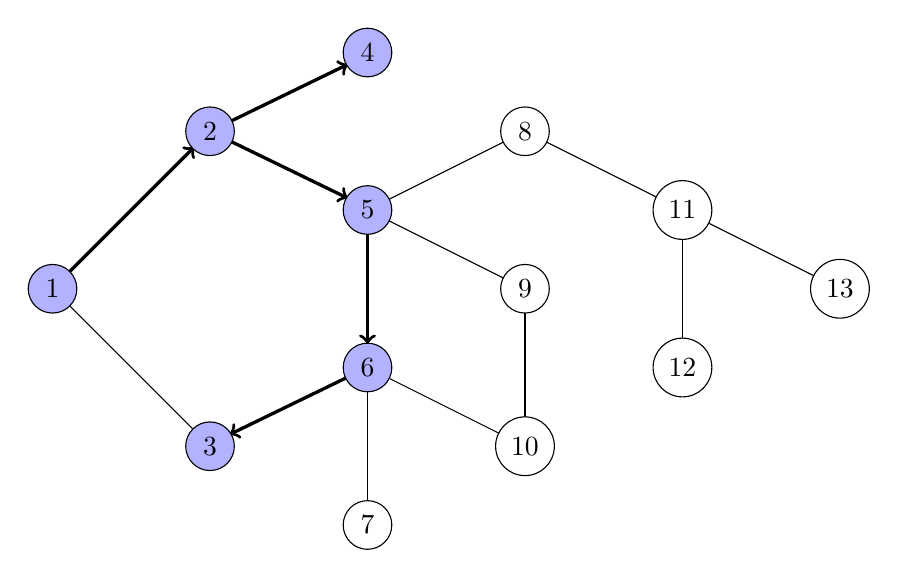
\begin{tikzpicture}
        \draw[very thick,->] (0,4) -- (1.8,5.8);
        \draw[very thick,->] (2,6) -- (3.75,6.85);
        \draw[very thick,->] (2,6) -- (3.75,5.15);
        \draw[very thick,->] (4,5) -- (4,3.3);
        \draw[very thick,->] (4,3) -- (2.25,2.15);
        \draw (0,4) -- (2,2);
        \draw (4,3) -- (4,1);
        \draw (4,3) -- (6,2);
        \draw (4,5) -- (6,6);
        \draw (4,5) -- (6,4);
        \draw (6,2) -- (6,4);
        \draw (6,6) -- (8,5);
        \draw (8,5) -- (8,3);
        \draw (8,5) -- (10,4);

        \node[circle, draw, fill=blue!30] at (0, 4) {1};
        \node[circle, draw, fill=blue!30] at (2, 6) {2};
        \node[circle, draw, fill=blue!30] at (2, 2) {3};
        \node[circle, draw, fill=blue!30] at (4, 7) {4};
        \node[circle, draw, fill=blue!30] at (4, 5) {5};
        \node[circle, draw, fill=blue!30] at (4, 3) {6};
        \node[circle, draw, fill=white] at (4, 1) {7};
        \node[circle, draw, fill=white] at (6, 6) {8};
        \node[circle, draw, fill=white] at (6, 4) {9};
        \node[circle, draw, fill=white] at (6, 2) {10};
        \node[circle, draw, fill=white] at (8, 5) {11};
        \node[circle, draw, fill=white] at (8, 3) {12};
        \node[circle, draw, fill=white] at (10, 4) {13};

    \end{tikzpicture}

\end{frame}

\begin{frame}[fragile]{Visualização da DFS}

    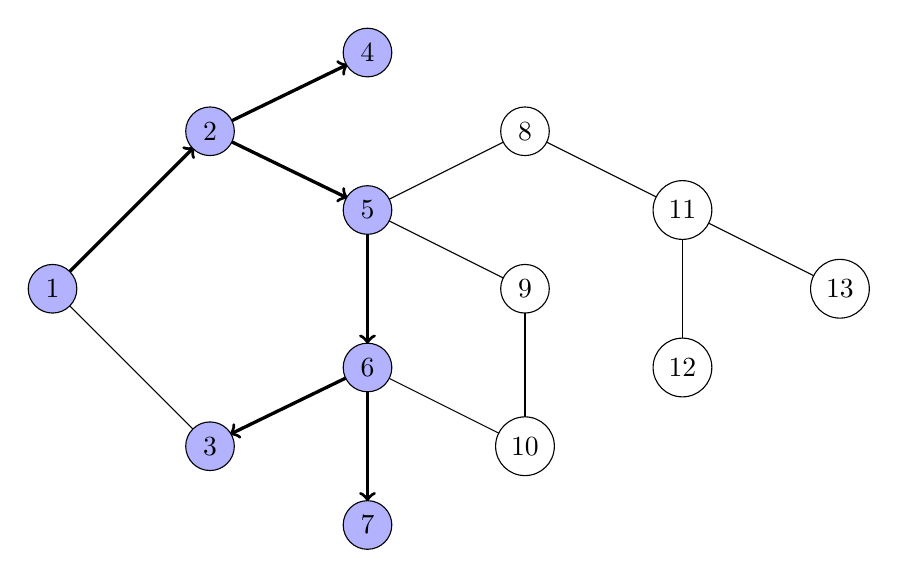
\begin{tikzpicture}
        \draw[very thick,->] (0,4) -- (1.8,5.8);
        \draw[very thick,->] (2,6) -- (3.75,6.85);
        \draw[very thick,->] (2,6) -- (3.75,5.15);
        \draw[very thick,->] (4,5) -- (4,3.3);
        \draw[very thick,->] (4,3) -- (2.25,2.15);
        \draw[very thick,->] (4,3) -- (4,1.3);
        \draw (0,4) -- (2,2);
        \draw (4,3) -- (6,2);
        \draw (4,5) -- (6,6);
        \draw (4,5) -- (6,4);
        \draw (6,2) -- (6,4);
        \draw (6,6) -- (8,5);
        \draw (8,5) -- (8,3);
        \draw (8,5) -- (10,4);

        \node[circle, draw, fill=blue!30] at (0, 4) {1};
        \node[circle, draw, fill=blue!30] at (2, 6) {2};
        \node[circle, draw, fill=blue!30] at (2, 2) {3};
        \node[circle, draw, fill=blue!30] at (4, 7) {4};
        \node[circle, draw, fill=blue!30] at (4, 5) {5};
        \node[circle, draw, fill=blue!30] at (4, 3) {6};
        \node[circle, draw, fill=blue!30] at (4, 1) {7};
        \node[circle, draw, fill=white] at (6, 6) {8};
        \node[circle, draw, fill=white] at (6, 4) {9};
        \node[circle, draw, fill=white] at (6, 2) {10};
        \node[circle, draw, fill=white] at (8, 5) {11};
        \node[circle, draw, fill=white] at (8, 3) {12};
        \node[circle, draw, fill=white] at (10, 4) {13};

    \end{tikzpicture}

\end{frame}

\begin{frame}[fragile]{Visualização da DFS}

    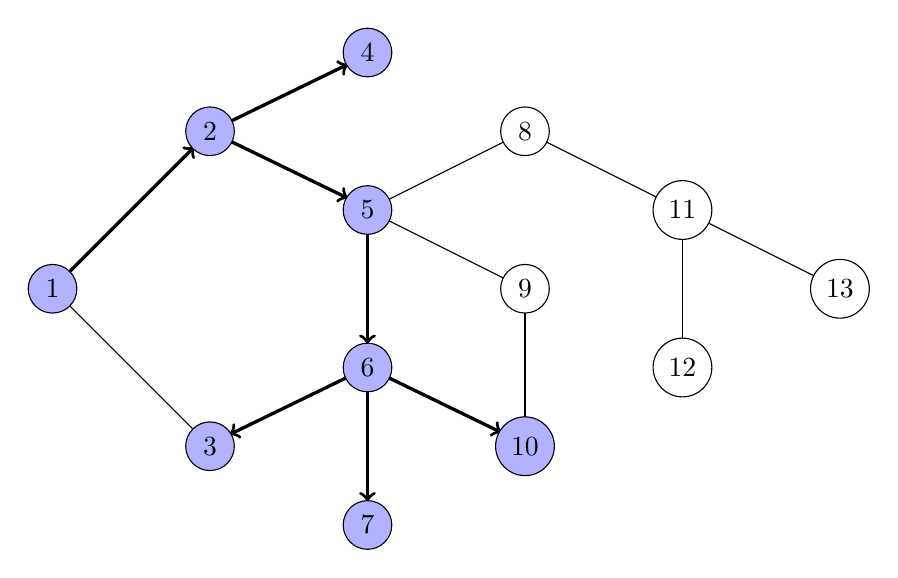
\begin{tikzpicture}
        \draw[very thick,->] (0,4) -- (1.8,5.8);
        \draw[very thick,->] (2,6) -- (3.75,6.85);
        \draw[very thick,->] (2,6) -- (3.75,5.15);
        \draw[very thick,->] (4,5) -- (4,3.3);
        \draw[very thick,->] (4,3) -- (2.25,2.15);
        \draw[very thick,->] (4,3) -- (4,1.3);
        \draw[very thick,->] (4,3) -- (5.70,2.175);
        \draw (0,4) -- (2,2);
        \draw (4,5) -- (6,6);
        \draw (4,5) -- (6,4);
        \draw (6,2) -- (6,4);
        \draw (6,6) -- (8,5);
        \draw (8,5) -- (8,3);
        \draw (8,5) -- (10,4);

        \node[circle, draw, fill=blue!30] at (0, 4) {1};
        \node[circle, draw, fill=blue!30] at (2, 6) {2};
        \node[circle, draw, fill=blue!30] at (2, 2) {3};
        \node[circle, draw, fill=blue!30] at (4, 7) {4};
        \node[circle, draw, fill=blue!30] at (4, 5) {5};
        \node[circle, draw, fill=blue!30] at (4, 3) {6};
        \node[circle, draw, fill=blue!30] at (4, 1) {7};
        \node[circle, draw, fill=white] at (6, 6) {8};
        \node[circle, draw, fill=white] at (6, 4) {9};
        \node[circle, draw, fill=blue!30] at (6, 2) {10};
        \node[circle, draw, fill=white] at (8, 5) {11};
        \node[circle, draw, fill=white] at (8, 3) {12};
        \node[circle, draw, fill=white] at (10, 4) {13};

    \end{tikzpicture}

\end{frame}

\begin{frame}[fragile]{Visualização da DFS}

    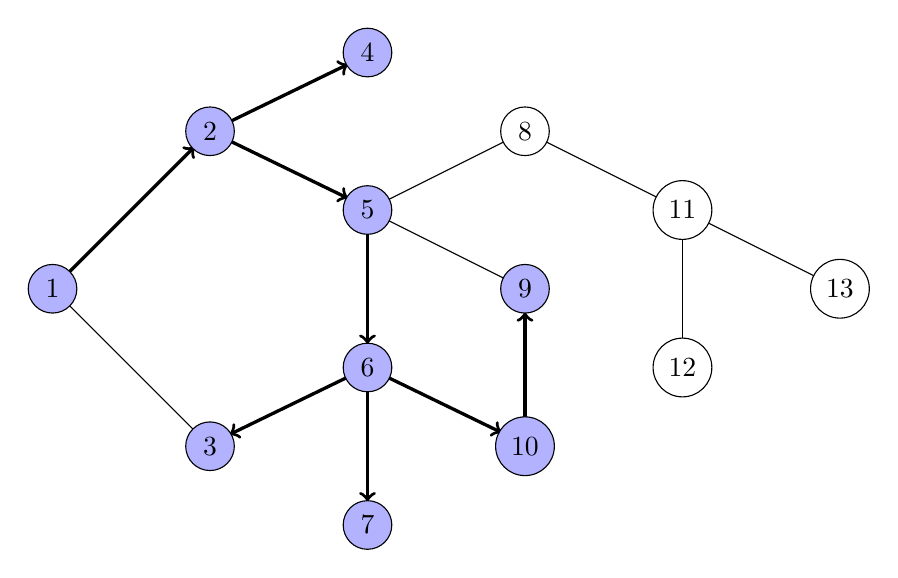
\begin{tikzpicture}
        \draw[very thick,->] (0,4) -- (1.8,5.8);
        \draw[very thick,->] (2,6) -- (3.75,6.85);
        \draw[very thick,->] (2,6) -- (3.75,5.15);
        \draw[very thick,->] (4,5) -- (4,3.3);
        \draw[very thick,->] (4,3) -- (2.25,2.15);
        \draw[very thick,->] (4,3) -- (4,1.3);
        \draw[very thick,->] (4,3) -- (5.70,2.175);
        \draw[very thick,->] (6,2) -- (6,3.7);
        \draw (0,4) -- (2,2);
        \draw (4,5) -- (6,6);
        \draw (4,5) -- (6,4);
        \draw (6,6) -- (8,5);
        \draw (8,5) -- (8,3);
        \draw (8,5) -- (10,4);

        \node[circle, draw, fill=blue!30] at (0, 4) {1};
        \node[circle, draw, fill=blue!30] at (2, 6) {2};
        \node[circle, draw, fill=blue!30] at (2, 2) {3};
        \node[circle, draw, fill=blue!30] at (4, 7) {4};
        \node[circle, draw, fill=blue!30] at (4, 5) {5};
        \node[circle, draw, fill=blue!30] at (4, 3) {6};
        \node[circle, draw, fill=blue!30] at (4, 1) {7};
        \node[circle, draw, fill=white] at (6, 6) {8};
        \node[circle, draw, fill=blue!30] at (6, 4) {9};
        \node[circle, draw, fill=blue!30] at (6, 2) {10};
        \node[circle, draw, fill=white] at (8, 5) {11};
        \node[circle, draw, fill=white] at (8, 3) {12};
        \node[circle, draw, fill=white] at (10, 4) {13};

    \end{tikzpicture}

\end{frame}

\begin{frame}[fragile]{Visualização da DFS}

    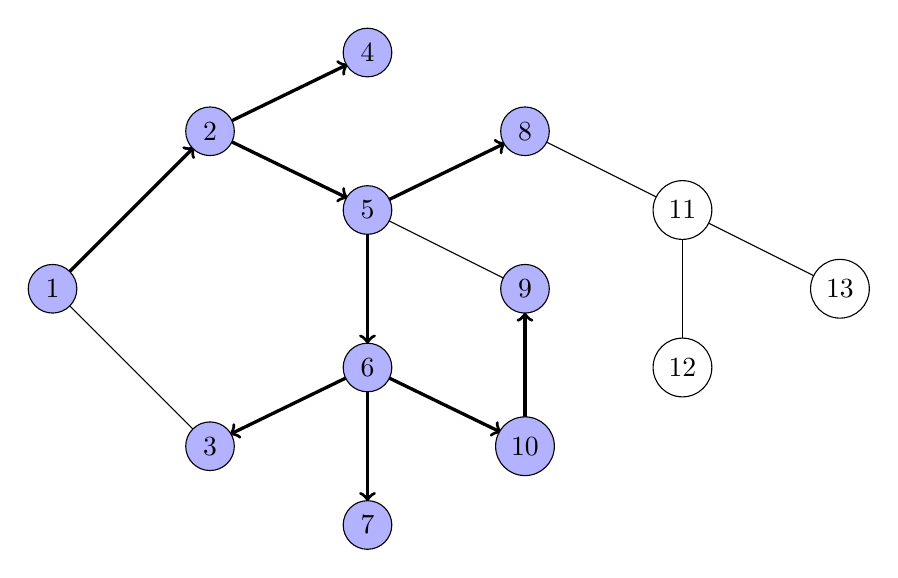
\begin{tikzpicture}
        \draw[very thick,->] (0,4) -- (1.8,5.8);
        \draw[very thick,->] (2,6) -- (3.75,6.85);
        \draw[very thick,->] (2,6) -- (3.75,5.15);
        \draw[very thick,->] (4,5) -- (4,3.3);
        \draw[very thick,->] (4,3) -- (2.25,2.15);
        \draw[very thick,->] (4,3) -- (4,1.3);
        \draw[very thick,->] (4,3) -- (5.70,2.175);
        \draw[very thick,->] (6,2) -- (6,3.7);
        \draw[very thick,->] (4,5) -- (5.75,5.85);
        \draw (0,4) -- (2,2);
        \draw (4,5) -- (6,4);
        \draw (6,6) -- (8,5);
        \draw (8,5) -- (8,3);
        \draw (8,5) -- (10,4);

        \node[circle, draw, fill=blue!30] at (0, 4) {1};
        \node[circle, draw, fill=blue!30] at (2, 6) {2};
        \node[circle, draw, fill=blue!30] at (2, 2) {3};
        \node[circle, draw, fill=blue!30] at (4, 7) {4};
        \node[circle, draw, fill=blue!30] at (4, 5) {5};
        \node[circle, draw, fill=blue!30] at (4, 3) {6};
        \node[circle, draw, fill=blue!30] at (4, 1) {7};
        \node[circle, draw, fill=blue!30] at (6, 6) {8};
        \node[circle, draw, fill=blue!30] at (6, 4) {9};
        \node[circle, draw, fill=blue!30] at (6, 2) {10};
        \node[circle, draw, fill=white] at (8, 5) {11};
        \node[circle, draw, fill=white] at (8, 3) {12};
        \node[circle, draw, fill=white] at (10, 4) {13};

    \end{tikzpicture}

\end{frame}

\begin{frame}[fragile]{Visualização da DFS}

    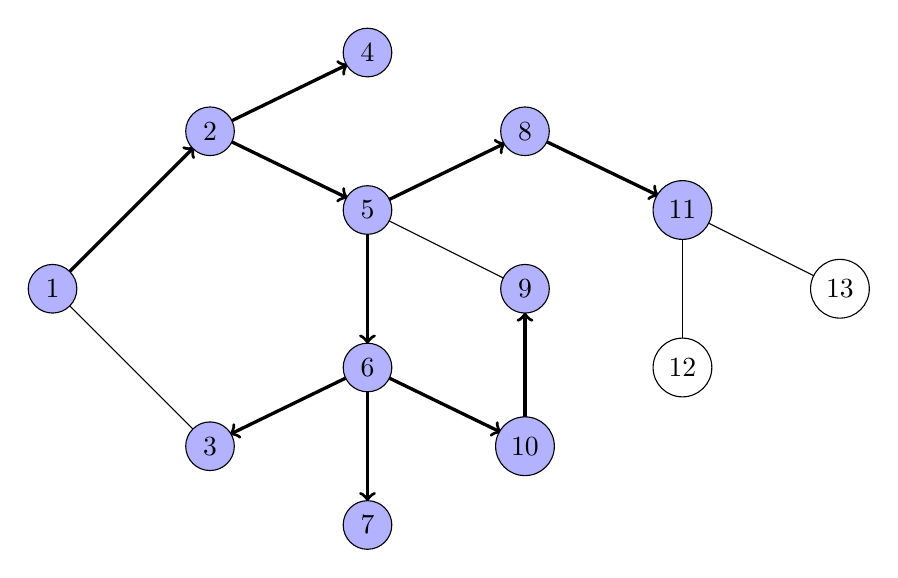
\begin{tikzpicture}
        \draw[very thick,->] (0,4) -- (1.8,5.8);
        \draw[very thick,->] (2,6) -- (3.75,6.85);
        \draw[very thick,->] (2,6) -- (3.75,5.15);
        \draw[very thick,->] (4,5) -- (4,3.3);
        \draw[very thick,->] (4,3) -- (2.25,2.15);
        \draw[very thick,->] (4,3) -- (4,1.3);
        \draw[very thick,->] (4,3) -- (5.70,2.175);
        \draw[very thick,->] (6,2) -- (6,3.7);
        \draw[very thick,->] (4,5) -- (5.75,5.85);
        \draw[very thick,->] (6,6) -- (7.7,5.18);
        \draw (0,4) -- (2,2);
        \draw (4,5) -- (6,4);
        \draw (8,5) -- (8,3);
        \draw (8,5) -- (10,4);

        \node[circle, draw, fill=blue!30] at (0, 4) {1};
        \node[circle, draw, fill=blue!30] at (2, 6) {2};
        \node[circle, draw, fill=blue!30] at (2, 2) {3};
        \node[circle, draw, fill=blue!30] at (4, 7) {4};
        \node[circle, draw, fill=blue!30] at (4, 5) {5};
        \node[circle, draw, fill=blue!30] at (4, 3) {6};
        \node[circle, draw, fill=blue!30] at (4, 1) {7};
        \node[circle, draw, fill=blue!30] at (6, 6) {8};
        \node[circle, draw, fill=blue!30] at (6, 4) {9};
        \node[circle, draw, fill=blue!30] at (6, 2) {10};
        \node[circle, draw, fill=blue!30] at (8, 5) {11};
        \node[circle, draw, fill=white] at (8, 3) {12};
        \node[circle, draw, fill=white] at (10, 4) {13};

    \end{tikzpicture}

\end{frame}

\begin{frame}[fragile]{Visualização da DFS}

    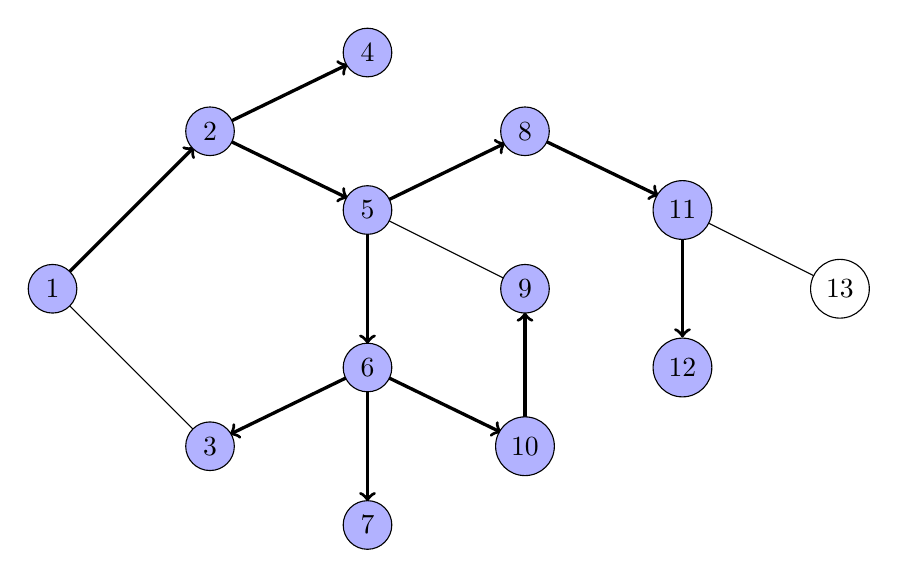
\begin{tikzpicture}
        \draw[very thick,->] (0,4) -- (1.8,5.8);
        \draw[very thick,->] (2,6) -- (3.75,6.85);
        \draw[very thick,->] (2,6) -- (3.75,5.15);
        \draw[very thick,->] (4,5) -- (4,3.3);
        \draw[very thick,->] (4,3) -- (2.25,2.15);
        \draw[very thick,->] (4,3) -- (4,1.3);
        \draw[very thick,->] (4,3) -- (5.70,2.175);
        \draw[very thick,->] (6,2) -- (6,3.7);
        \draw[very thick,->] (4,5) -- (5.75,5.85);
        \draw[very thick,->] (6,6) -- (7.7,5.18);
        \draw[very thick,->] (8,5) -- (8,3.38);
        \draw (0,4) -- (2,2);
        \draw (4,5) -- (6,4);
        \draw (8,5) -- (10,4);

        \node[circle, draw, fill=blue!30] at (0, 4) {1};
        \node[circle, draw, fill=blue!30] at (2, 6) {2};
        \node[circle, draw, fill=blue!30] at (2, 2) {3};
        \node[circle, draw, fill=blue!30] at (4, 7) {4};
        \node[circle, draw, fill=blue!30] at (4, 5) {5};
        \node[circle, draw, fill=blue!30] at (4, 3) {6};
        \node[circle, draw, fill=blue!30] at (4, 1) {7};
        \node[circle, draw, fill=blue!30] at (6, 6) {8};
        \node[circle, draw, fill=blue!30] at (6, 4) {9};
        \node[circle, draw, fill=blue!30] at (6, 2) {10};
        \node[circle, draw, fill=blue!30] at (8, 5) {11};
        \node[circle, draw, fill=blue!30] at (8, 3) {12};
        \node[circle, draw, fill=white] at (10, 4) {13};

    \end{tikzpicture}

\end{frame}

\begin{frame}[fragile]{Visualização da DFS}

    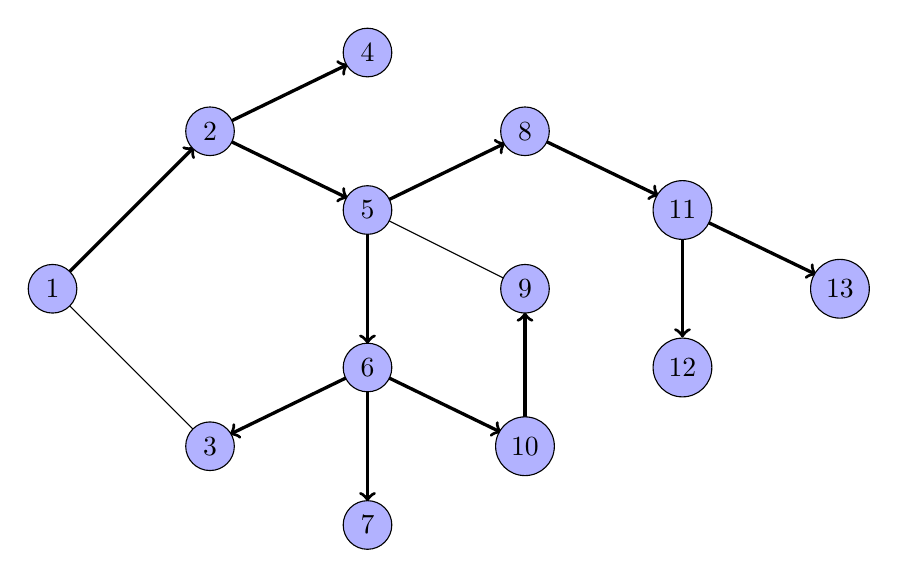
\begin{tikzpicture}
        \draw[very thick,->] (0,4) -- (1.8,5.8);
        \draw[very thick,->] (2,6) -- (3.75,6.85);
        \draw[very thick,->] (2,6) -- (3.75,5.15);
        \draw[very thick,->] (4,5) -- (4,3.3);
        \draw[very thick,->] (4,3) -- (2.25,2.15);
        \draw[very thick,->] (4,3) -- (4,1.3);
        \draw[very thick,->] (4,3) -- (5.70,2.175);
        \draw[very thick,->] (6,2) -- (6,3.7);
        \draw[very thick,->] (4,5) -- (5.75,5.85);
        \draw[very thick,->] (6,6) -- (7.7,5.18);
        \draw[very thick,->] (8,5) -- (8,3.38);
        \draw[very thick,->] (8,5) -- (9.7,4.18);
        \draw (0,4) -- (2,2);
        \draw (4,5) -- (6,4);

        \node[circle, draw, fill=blue!30] at (0, 4) {1};
        \node[circle, draw, fill=blue!30] at (2, 6) {2};
        \node[circle, draw, fill=blue!30] at (2, 2) {3};
        \node[circle, draw, fill=blue!30] at (4, 7) {4};
        \node[circle, draw, fill=blue!30] at (4, 5) {5};
        \node[circle, draw, fill=blue!30] at (4, 3) {6};
        \node[circle, draw, fill=blue!30] at (4, 1) {7};
        \node[circle, draw, fill=blue!30] at (6, 6) {8};
        \node[circle, draw, fill=blue!30] at (6, 4) {9};
        \node[circle, draw, fill=blue!30] at (6, 2) {10};
        \node[circle, draw, fill=blue!30] at (8, 5) {11};
        \node[circle, draw, fill=blue!30] at (8, 3) {12};
        \node[circle, draw, fill=blue!30] at (10, 4) {13};

    \end{tikzpicture}

\end{frame}

\section{Implementação}

\begin{frame}[fragile]{Implementação da DFS em C++}
    \inputsnippet{c++}{1}{21}{dfs.cpp}
\end{frame}

\begin{frame}[fragile]{Implementação da DFS em C++}
    \inputsnippet{c++}{23}{43}{dfs.cpp}
\end{frame}
